\documentclass[tikz,border=1pt]{standalone}
\usepackage{fontspec,xeCJK,amsmath,amssymb,lmodern,graphicx}
\setmainfont{Comic Sans MS}
\setCJKmainfont{Microsoft YaHei}
\usetikzlibrary{arrows.meta,calc}
\tikzset{every node/.style={inner sep=0pt,outer sep=0pt,align=center}}
\definecolor{Ink}{HTML}{25282D}
\definecolor{Muted}{HTML}{53575E}
\definecolor{Line}{HTML}{BAC8C9}
\definecolor{Blue}{HTML}{5975A2}
\definecolor{BlueLight}{HTML}{DCE5F4}
\definecolor{BlueBg}{HTML}{FFFFFF}
\definecolor{Orange}{HTML}{DC8650}
\definecolor{OrangeLight}{HTML}{FFE0A7}
\definecolor{OrangeBg}{HTML}{FFF8F0}
\definecolor{Green}{HTML}{76896B}
\definecolor{GreenLight}{HTML}{E7EFDF}
\definecolor{GreenBg}{HTML}{FFFFFF}
\definecolor{White}{HTML}{FFFFFF}
\definecolor{Gray}{HTML}{DCE4E5}
\definecolor{Soft}{HTML}{F8FAFA}
\definecolor{BlueSide}{HTML}{B6C6E2}
\definecolor{BlueTop}{HTML}{F0F4FB}
\definecolor{BlueBorder}{HTML}{ABBBD3}
\definecolor{BlueHatch}{HTML}{E5EFF8}
\definecolor{GreenSide}{HTML}{CEDDC1}
\definecolor{GreenTop}{HTML}{F5F8EF}
\definecolor{GreenBorder}{HTML}{BAC9AE}
\definecolor{GreenHatch}{HTML}{EAF2DF}
\definecolor{Rose}{HTML}{AE734D}
\definecolor{RoseLight}{HTML}{F8DFCB}
\definecolor{RoseBg}{HTML}{FFFFFF}
\definecolor{RoseSide}{HTML}{E9BFA0}
\definecolor{RoseTop}{HTML}{FFF2E7}
\definecolor{RoseBorder}{HTML}{D8B79E}
\definecolor{RoseHatch}{HTML}{FAEBE8}
\definecolor{Flow}{HTML}{51545B}
\definecolor{Snow}{HTML}{6993B5}
\definecolor{Cream}{HTML}{FFF8EE}
\definecolor{CreamLine}{HTML}{DDB993}
\definecolor{Feature}{HTML}{B3D9CD}
\definecolor{FeatureDark}{HTML}{78AF9D}
\definecolor{Source}{HTML}{6688AA}
\definecolor{SourceLight}{HTML}{DCE9F4}
\definecolor{SourceTop}{HTML}{F4F8FC}
\definecolor{SourceSide}{HTML}{B8CBDF}
\definecolor{SourceBg}{HTML}{F4F7FB}
\definecolor{History}{HTML}{747EAF}
\definecolor{HistoryLight}{HTML}{E4E7F5}
\definecolor{HistoryTop}{HTML}{F6F7FC}
\definecolor{HistorySide}{HTML}{C5CBE6}
\definecolor{HistoryBg}{HTML}{F6F6FB}
\definecolor{Target}{HTML}{5878AD}
\definecolor{TargetLight}{HTML}{E7EDF9}
\definecolor{TargetTop}{HTML}{F4F7FD}
\definecolor{TargetSide}{HTML}{B8C8E5}
\definecolor{Loss}{HTML}{3B789F}
\definecolor{LossLight}{HTML}{EBF4FA}
\definecolor{LossTop}{HTML}{F7FBFD}
\definecolor{LossSide}{HTML}{C4DBEA}
\definecolor{Step}{HTML}{3D5B8A}
\definecolor{StepLight}{HTML}{BDCCE6}
\definecolor{StepTop}{HTML}{E7EDF8}
\definecolor{StepSide}{HTML}{91ABD2}
\definecolor{CyanCell0}{HTML}{EFF5FA}
\definecolor{CyanCell1}{HTML}{DCE8F4}
\definecolor{CyanCell2}{HTML}{B9CDE4}
\definecolor{CyanCell3}{HTML}{8DAACF}
\definecolor{CyanCell4}{HTML}{6588BA}
\definecolor{IndigoCell0}{HTML}{F0F1F9}
\definecolor{IndigoCell1}{HTML}{DDE1F2}
\definecolor{IndigoCell2}{HTML}{B9C3E3}
\definecolor{IndigoCell3}{HTML}{94A3CE}
\definecolor{IndigoCell4}{HTML}{7387BC}
\definecolor{GradCell0}{HTML}{C7DFEF}
\definecolor{GradCell1}{HTML}{6EA2CE}
\definecolor{GradCell2}{HTML}{315F96}
\definecolor{Grad}{HTML}{327D73}
\definecolor{GradBg}{HTML}{F0F8F4}
\definecolor{GradBorder}{HTML}{9FC6B8}
\definecolor{GradLight}{HTML}{D8EDE3}
\definecolor{GradMid}{HTML}{91C7B2}
\definecolor{Update}{HTML}{668346}
\definecolor{UpdateBg}{HTML}{F4F8EA}
\definecolor{UpdateBorder}{HTML}{B1C58F}
\definecolor{UpdateLight}{HTML}{E1EDCB}
\definecolor{Calib}{HTML}{81906D}
\definecolor{CalibLight}{HTML}{E6EEDB}
\definecolor{CalibTop}{HTML}{F5F8EF}
\definecolor{CalibSide}{HTML}{CDDAB9}
\definecolor{CalibBg}{HTML}{F8FAF4}
\definecolor{CalibBorder}{HTML}{B9C6AA}
\definecolor{Feedback}{HTML}{678D7D}
\definecolor{FeedbackLight}{HTML}{E4EFE8}
\definecolor{FeedbackTop}{HTML}{F4F9F6}
\definecolor{FeedbackSide}{HTML}{B9D3C5}
\definecolor{FeedbackBg}{HTML}{F5F9F6}
\definecolor{FeedbackBorder}{HTML}{BACFC2}
\definecolor{Shared}{HTML}{A56C45}
\definecolor{SharedLight}{HTML}{F0CFB5}
\definecolor{SharedTop}{HTML}{FFF0E4}
\definecolor{SharedSide}{HTML}{DBAF8C}
\definecolor{Berry0}{HTML}{FBEDE2}
\definecolor{Berry1}{HTML}{F5DBCA}
\definecolor{Berry2}{HTML}{EAC2A4}
\definecolor{Berry3}{HTML}{D6A27A}
\definecolor{Berry4}{HTML}{BA8259}
\definecolor{Mint0}{HTML}{E7F1EB}
\definecolor{Mint1}{HTML}{CEDFD5}
\definecolor{Mint2}{HTML}{A0C0AE}
\definecolor{Mint3}{HTML}{759F88}
\definecolor{FormulaBg}{HTML}{F1F5FC}
\definecolor{FormulaBorder}{HTML}{B1C1DB}
\definecolor{GroupB}{HTML}{C58C64}
\definecolor{GroupA}{HTML}{839BC5}
\definecolor{PanelLine}{HTML}{696C71}
\definecolor{PanelShadow}{HTML}{EAEAEA}
\definecolor{GroupBBg}{HTML}{FFFCF9}
\definecolor{GroupABg}{HTML}{FCFDFF}
\definecolor{SlabFace}{HTML}{B9CAE8}
\definecolor{SlabTop}{HTML}{EDF2FB}
\definecolor{SlabSide}{HTML}{92A9CF}
\definecolor{SlabEdge}{HTML}{B5C3D9}
\begin{document}
\begin{tikzpicture}[x=1cm,y=-1cm]
\path[use as bounding box] (0,0) rectangle (18.0,10.7);
\draw[fill=PanelShadow,draw=PanelShadow,line width=0pt,rounded corners=0.31cm] (0.155,0.16499999999999998) rectangle (17.915000000000003,4.865);
\draw[fill=White,draw=PanelLine,line width=0.62pt,rounded corners=0.31cm] (0.12,0.12) rectangle (17.880000000000003,4.82);
\node[text=Ink,font=\fontsize{9.3}{11.0}\selectfont\bfseries] (n2) at (2.6706294736842104,0.46) {(a) Federated LoRA training};
\path let \p1=($(n2.east)-(n2.west)$), \p2=($(n2.north)-(n2.south)$) in \pgfextra{\typeout{SIZE|2|\x1|\y2}};
\draw[fill=GroupBBg,draw=GroupB,line width=0.52pt,dash pattern=on 2.4pt off 1.8pt,rounded corners=0.14cm] (0.55,0.85) rectangle (6.1499999999999995,3.98);
\draw[fill=GroupABg,draw=GroupA,line width=0.52pt,dash pattern=on 2.4pt off 1.8pt,rounded corners=0.14cm] (12.16,0.85) rectangle (17.58,3.98);
\node[text=Ink,font=\fontsize{8.8}{10.5}\selectfont\bfseries] (n5) at (3.35,1.12) {Client: B training};
\path let \p1=($(n5.east)-(n5.west)$), \p2=($(n5.north)-(n5.south)$) in \pgfextra{\typeout{SIZE|5|\x1|\y2}};
\node[text=Muted,font=\fontsize{8.3}{10.0}\selectfont] (n6) at (3.1399999999999997,1.5099999999999998) {LoRA};
\path let \p1=($(n6.east)-(n6.west)$), \p2=($(n6.north)-(n6.south)$) in \pgfextra{\typeout{SIZE|6|\x1|\y2}};
\draw[fill=BlueTop,draw=Blue,line width=0.35pt,line join=round] (2.32,1.91) -- (2.4299999999999997,1.7999999999999998) -- (3.05,1.7999999999999998) -- (2.94,1.91) -- cycle;
\draw[fill=BlueSide,draw=Blue,line width=0.35pt,line join=round] (2.94,1.91) -- (3.05,1.7999999999999998) -- (3.05,2.23) -- (2.94,2.34) -- cycle;
\draw[fill=BlueLight,draw=Blue,line width=0.45pt] (2.32,1.91) rectangle (2.94,2.34);
\node[text=Ink,font=\fontsize{10.0}{11.7}\selectfont] (n10) at (2.63,2.125) {A};
\path let \p1=($(n10.east)-(n10.west)$), \p2=($(n10.north)-(n10.south)$) in \pgfextra{\typeout{SIZE|10|\x1|\y2}};
\draw[draw=White,line width=0.48pt,line join=round] (2.3449999999999998,1.9349999999999998) -- (2.915,1.9349999999999998);
\draw[draw=White,line width=0.48pt,line join=round] (2.3449999999999998,1.9349999999999998) -- (2.3449999999999998,2.315);
\draw[draw=Snow,line width=0.7pt,line join=round] (2.8449999999999998,1.79) -- (3.035,1.79);
\draw[draw=Snow,line width=0.48pt,line join=round] (2.87825,1.79) -- (2.9024330519165797,1.76581694808342);
\draw[draw=Snow,line width=0.48pt,line join=round] (2.87825,1.79) -- (2.9024330519165797,1.81418305191658);
\draw[draw=Snow,line width=0.48pt,line join=round] (3.00175,1.79) -- (2.97756694808342,1.81418305191658);
\draw[draw=Snow,line width=0.48pt,line join=round] (3.00175,1.79) -- (2.97756694808342,1.76581694808342);
\draw[draw=Snow,line width=0.7pt,line join=round] (2.8925,1.7077275866404784) -- (2.9875,1.8722724133595217);
\draw[draw=Snow,line width=0.48pt,line join=round] (2.909125,1.7365229313163109) -- (2.942159663259086,1.745374542658817);
\draw[draw=Snow,line width=0.48pt,line join=round] (2.909125,1.7365229313163109) -- (2.9002733886574936,1.769557594575397);
\draw[draw=Snow,line width=0.48pt,line join=round] (2.970875,1.8434770686836892) -- (2.937840336740914,1.834625457341183);
\draw[draw=Snow,line width=0.48pt,line join=round] (2.970875,1.8434770686836892) -- (2.9797266113425063,1.810442405424603);
\draw[draw=Snow,line width=0.7pt,line join=round] (2.9875,1.7077275866404784) -- (2.8925,1.8722724133595217);
\draw[draw=Snow,line width=0.48pt,line join=round] (2.970875,1.7365229313163109) -- (2.9797266113425063,1.769557594575397);
\draw[draw=Snow,line width=0.48pt,line join=round] (2.970875,1.7365229313163109) -- (2.937840336740914,1.745374542658817);
\draw[draw=Snow,line width=0.48pt,line join=round] (2.909125,1.8434770686836892) -- (2.9002733886574936,1.810442405424603);
\draw[draw=Snow,line width=0.48pt,line join=round] (2.909125,1.8434770686836892) -- (2.942159663259086,1.834625457341183);
\draw[fill=RoseTop,draw=Rose,line width=0.35pt,line join=round] (3.34,1.91) -- (3.4499999999999997,1.7999999999999998) -- (4.07,1.7999999999999998) -- (3.96,1.91) -- cycle;
\draw[fill=RoseSide,draw=Rose,line width=0.35pt,line join=round] (3.96,1.91) -- (4.07,1.7999999999999998) -- (4.07,2.23) -- (3.96,2.34) -- cycle;
\draw[fill=RoseLight,draw=Rose,line width=0.45pt] (3.34,1.91) rectangle (3.96,2.34);
\node[text=Ink,font=\fontsize{10.0}{11.7}\selectfont] (n31) at (3.65,2.125) {B};
\path let \p1=($(n31.east)-(n31.west)$), \p2=($(n31.north)-(n31.south)$) in \pgfextra{\typeout{SIZE|31|\x1|\y2}};
\draw[draw=White,line width=0.48pt,line join=round] (3.3649999999999998,1.9349999999999998) -- (3.935,1.9349999999999998);
\draw[draw=White,line width=0.48pt,line join=round] (3.3649999999999998,1.9349999999999998) -- (3.3649999999999998,2.315);
\draw[fill=Orange,draw=Orange,line width=0.3pt,line join=round] (3.9495,1.685) -- (3.981,1.7585) -- (4.0125,1.7217500000000001) -- (4.04925,1.8005) -- (4.03875,1.85825) -- (3.99675,1.895) -- (3.9285,1.895) -- (3.88125,1.85825) -- (3.876,1.8005) -- (3.91275,1.748) -- (3.918,1.811) -- (3.96,1.7585) -- cycle;
\draw[fill=OrangeLight,draw=OrangeLight,line width=0.15pt,line join=round] (3.93375,1.874) -- (3.98625,1.874) -- (3.9768,1.8215000000000001) -- (3.96,1.83725) -- (3.9558,1.7921) -- cycle;
\node at (1.15,2.8000000000000003) {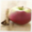
\includegraphics[width=0.4cm,height=0.4cm]{assets/apple.png}};
\node at (1.42,2.68) {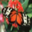
\includegraphics[width=0.4cm,height=0.4cm]{assets/butterfly.png}};
\draw[fill=GreenLight,draw=Green,line width=0.45pt,rounded corners=0.025cm] (0.91,3.06) rectangle (1.73,3.24);
\node[text=Muted,font=\fontsize{8.3}{10.0}\selectfont] (n39) at (1.32,3.57) {Images\\+ text};
\path let \p1=($(n39.east)-(n39.west)$), \p2=($(n39.north)-(n39.south)$) in \pgfextra{\typeout{SIZE|39|\x1|\y2}};
\draw[draw=Flow,line width=0.7pt,line join=round,-{Stealth[length=3.7pt,width=3pt]}] (1.77,2.89) -- (2.55,2.89);
\draw[fill=SlabTop,draw=SlabEdge,line width=0.25pt,line join=round] (2.6681250000000003,2.5225) -- (2.7618750000000003,2.42875) -- (2.961875,2.42875) -- (2.8681250000000005,2.5225) -- cycle;
\draw[fill=SlabSide,draw=SlabEdge,line width=0.25pt,line join=round] (2.8681250000000005,2.5225) -- (2.961875,2.42875) -- (2.961875,3.2037500000000003) -- (2.8681250000000005,3.2975000000000003) -- cycle;
\draw[fill=SlabFace,draw=White,line width=0.52pt] (2.6681250000000003,2.5225) rectangle (2.8681250000000005,3.2975);
\draw[fill=SlabTop,draw=SlabEdge,line width=0.25pt,line join=round] (2.9931250000000005,2.66) -- (3.0868750000000005,2.56625) -- (3.286875,2.56625) -- (3.193125,2.66) -- cycle;
\draw[fill=SlabSide,draw=SlabEdge,line width=0.25pt,line join=round] (3.193125,2.66) -- (3.286875,2.56625) -- (3.286875,3.06625) -- (3.193125,3.16) -- cycle;
\draw[fill=SlabFace,draw=White,line width=0.52pt] (2.9931250000000005,2.66) rectangle (3.1931250000000007,3.16);
\draw[fill=SlabTop,draw=SlabEdge,line width=0.25pt,line join=round] (3.318125,2.5225) -- (3.411875,2.42875) -- (3.6118750000000004,2.42875) -- (3.5181250000000004,2.5225) -- cycle;
\draw[fill=SlabSide,draw=SlabEdge,line width=0.25pt,line join=round] (3.5181250000000004,2.5225) -- (3.6118750000000004,2.42875) -- (3.6118750000000004,3.2037500000000003) -- (3.5181250000000004,3.2975000000000003) -- cycle;
\draw[fill=SlabFace,draw=White,line width=0.52pt] (3.318125,2.5225) rectangle (3.5181250000000004,3.2975);
\draw[draw=Snow,line width=0.7pt,line join=round] (2.786875,2.4850000000000003) -- (2.974375,2.4850000000000003);
\draw[draw=Snow,line width=0.48pt,line join=round] (2.8196875,2.4850000000000003) -- (2.843552353865046,2.4611351461349544);
\draw[draw=Snow,line width=0.48pt,line join=round] (2.8196875,2.4850000000000003) -- (2.843552353865046,2.508864853865046);
\draw[draw=Snow,line width=0.48pt,line join=round] (2.9415625000000003,2.4850000000000003) -- (2.9176976461349544,2.508864853865046);
\draw[draw=Snow,line width=0.48pt,line join=round] (2.9415625000000003,2.4850000000000003) -- (2.9176976461349544,2.4611351461349544);
\draw[draw=Snow,line width=0.7pt,line join=round] (2.83375,2.403810118395209) -- (2.9275,2.5661898816047914);
\draw[draw=Snow,line width=0.48pt,line join=round] (2.8501562500000004,2.4322265769568863) -- (2.8827562466372565,2.4409617197290965);
\draw[draw=Snow,line width=0.48pt,line join=round] (2.8501562500000004,2.4322265769568863) -- (2.84142110722779,2.4648265735941424);
\draw[draw=Snow,line width=0.48pt,line join=round] (2.91109375,2.5377734230431144) -- (2.878493753362744,2.529038280270904);
\draw[draw=Snow,line width=0.48pt,line join=round] (2.91109375,2.5377734230431144) -- (2.9198288927722102,2.5051734264058583);
\draw[draw=Snow,line width=0.7pt,line join=round] (2.9275,2.403810118395209) -- (2.83375,2.5661898816047914);
\draw[draw=Snow,line width=0.48pt,line join=round] (2.91109375,2.4322265769568863) -- (2.9198288927722102,2.4648265735941424);
\draw[draw=Snow,line width=0.48pt,line join=round] (2.91109375,2.4322265769568863) -- (2.878493753362744,2.4409617197290965);
\draw[draw=Snow,line width=0.48pt,line join=round] (2.8501562500000004,2.5377734230431144) -- (2.84142110722779,2.5051734264058583);
\draw[draw=Snow,line width=0.48pt,line join=round] (2.8501562500000004,2.5377734230431144) -- (2.8827562466372565,2.529038280270904);
\node[text=Muted,font=\fontsize{8.3}{10.0}\selectfont] (n65) at (3.14,3.57) {CLIP};
\path let \p1=($(n65.east)-(n65.west)$), \p2=($(n65.north)-(n65.south)$) in \pgfextra{\typeout{SIZE|65|\x1|\y2}};
\draw[draw=Flow,line width=0.7pt,line join=round,-{Stealth[length=3.7pt,width=3pt]}] (3.17,2.25) -- (3.17,2.52);
\draw[draw=Flow,line width=0.7pt,line join=round,-{Stealth[length=3.7pt,width=3pt]}] (3.77,2.9) -- (4.54,2.9);
\draw[draw=Muted,line width=0.5pt,line join=round] (4.58,3.17) -- (5.62,3.17);
\draw[fill=GreenLight,draw=Green,line width=0.52pt] (4.68,2.98) rectangle (4.83,3.17);
\draw[fill=GreenLight,draw=Green,line width=0.52pt] (4.91,2.66) rectangle (5.0600000000000005,3.17);
\draw[fill=GreenLight,draw=Green,line width=0.52pt] (5.14,2.86) rectangle (5.29,3.17);
\draw[fill=GreenLight,draw=Green,line width=0.52pt] (5.37,3.05) rectangle (5.5200000000000005,3.17);
\node[text=Muted,font=\fontsize{8.3}{10.0}\selectfont] (n73) at (5.13,3.57) {Predictions};
\path let \p1=($(n73.east)-(n73.west)$), \p2=($(n73.north)-(n73.south)$) in \pgfextra{\typeout{SIZE|73|\x1|\y2}};
\node[text=Ink,font=\fontsize{8.8}{10.5}\selectfont\bfseries] (n74) at (9.1,1.12) {Aggregation};
\path let \p1=($(n74.east)-(n74.west)$), \p2=($(n74.north)-(n74.south)$) in \pgfextra{\typeout{SIZE|74|\x1|\y2}};
\draw[fill=GreenTop,draw=Green,line width=0.35pt,line join=round] (8.73,1.58) -- (8.8,1.51) -- (9.520000000000001,1.51) -- (9.450000000000001,1.58) -- cycle;
\draw[fill=GreenSide,draw=Green,line width=0.35pt,line join=round] (9.450000000000001,1.58) -- (9.520000000000001,1.51) -- (9.520000000000001,1.67) -- (9.450000000000001,1.74) -- cycle;
\draw[fill=GreenLight,draw=Green,line width=0.45pt] (8.73,1.58) rectangle (9.450000000000001,1.74);
\draw[draw=White,line width=0.48pt,line join=round] (8.755,1.605) -- (9.425,1.605);
\draw[draw=White,line width=0.48pt,line join=round] (8.755,1.605) -- (8.755,1.715);
\draw[fill=FeatureDark,draw=Green,line width=0.2pt] (8.83,1.6600000000000001) ellipse (0.0225cm and 0.0225cm);
\draw[fill=FeatureDark,draw=Green,line width=0.2pt] (8.94,1.6600000000000001) ellipse (0.0225cm and 0.0225cm);
\draw[draw=Green,line width=0.4pt,line join=round] (9.1,1.635) -- (9.35,1.635);
\draw[draw=Green,line width=0.4pt,line join=round] (9.1,1.685) -- (9.35,1.685);
\draw[fill=GreenTop,draw=Green,line width=0.35pt,line join=round] (8.73,1.8) -- (8.8,1.73) -- (9.520000000000001,1.73) -- (9.450000000000001,1.8) -- cycle;
\draw[fill=GreenSide,draw=Green,line width=0.35pt,line join=round] (9.450000000000001,1.8) -- (9.520000000000001,1.73) -- (9.520000000000001,1.89) -- (9.450000000000001,1.96) -- cycle;
\draw[fill=GreenLight,draw=Green,line width=0.45pt] (8.73,1.8) rectangle (9.450000000000001,1.96);
\draw[draw=White,line width=0.48pt,line join=round] (8.755,1.825) -- (9.425,1.825);
\draw[draw=White,line width=0.48pt,line join=round] (8.755,1.825) -- (8.755,1.935);
\draw[fill=FeatureDark,draw=Green,line width=0.2pt] (8.83,1.8800000000000001) ellipse (0.0225cm and 0.0225cm);
\draw[fill=FeatureDark,draw=Green,line width=0.2pt] (8.94,1.8800000000000001) ellipse (0.0225cm and 0.0225cm);
\draw[draw=Green,line width=0.4pt,line join=round] (9.1,1.855) -- (9.35,1.855);
\draw[draw=Green,line width=0.4pt,line join=round] (9.1,1.905) -- (9.35,1.905);
\draw[fill=GreenTop,draw=Green,line width=0.35pt,line join=round] (8.73,2.02) -- (8.8,1.95) -- (9.520000000000001,1.95) -- (9.450000000000001,2.02) -- cycle;
\draw[fill=GreenSide,draw=Green,line width=0.35pt,line join=round] (9.450000000000001,2.02) -- (9.520000000000001,1.95) -- (9.520000000000001,2.1100000000000003) -- (9.450000000000001,2.18) -- cycle;
\draw[fill=GreenLight,draw=Green,line width=0.45pt] (8.73,2.02) rectangle (9.450000000000001,2.18);
\draw[draw=White,line width=0.48pt,line join=round] (8.755,2.045) -- (9.425,2.045);
\draw[draw=White,line width=0.48pt,line join=round] (8.755,2.045) -- (8.755,2.1550000000000002);
\draw[fill=FeatureDark,draw=Green,line width=0.2pt] (8.83,2.1) ellipse (0.0225cm and 0.0225cm);
\draw[fill=FeatureDark,draw=Green,line width=0.2pt] (8.94,2.1) ellipse (0.0225cm and 0.0225cm);
\draw[draw=Green,line width=0.4pt,line join=round] (9.1,2.075) -- (9.35,2.075);
\draw[draw=Green,line width=0.4pt,line join=round] (9.1,2.125) -- (9.35,2.125);
\draw[fill=GreenLight,draw=Green,line width=0.52pt] (7.12,2.72) rectangle (7.6,3.0100000000000002);
\draw[fill=GreenSide,draw=Green,line width=0.6pt] (7.36,3.0100000000000002) ellipse (0.24cm and 0.07cm);
\draw[fill=GreenLight,draw=Green,line width=0.55pt] (7.36,2.8186) ellipse (0.24cm and 0.07cm);
\draw[fill=GreenLight,draw=Green,line width=0.55pt] (7.36,2.9143000000000003) ellipse (0.24cm and 0.07cm);
\draw[fill=GreenTop,draw=Green,line width=0.65pt] (7.36,2.72) ellipse (0.24cm and 0.07cm);
\node[text=Muted,font=\fontsize{8.3}{10.0}\selectfont] (n107) at (7.36,3.29) {Client 1};
\path let \p1=($(n107.east)-(n107.west)$), \p2=($(n107.north)-(n107.south)$) in \pgfextra{\typeout{SIZE|107|\x1|\y2}};
\draw[fill=GreenLight,draw=Green,line width=0.52pt] (8.86,2.72) rectangle (9.34,3.0100000000000002);
\draw[fill=GreenSide,draw=Green,line width=0.6pt] (9.1,3.0100000000000002) ellipse (0.24cm and 0.07cm);
\draw[fill=GreenLight,draw=Green,line width=0.55pt] (9.1,2.8186) ellipse (0.24cm and 0.07cm);
\draw[fill=GreenLight,draw=Green,line width=0.55pt] (9.1,2.9143000000000003) ellipse (0.24cm and 0.07cm);
\draw[fill=GreenTop,draw=Green,line width=0.65pt] (9.1,2.72) ellipse (0.24cm and 0.07cm);
\node[text=Muted,font=\fontsize{8.3}{10.0}\selectfont] (n113) at (9.1,3.29) {Client k};
\path let \p1=($(n113.east)-(n113.west)$), \p2=($(n113.north)-(n113.south)$) in \pgfextra{\typeout{SIZE|113|\x1|\y2}};
\draw[fill=GreenLight,draw=Green,line width=0.52pt] (10.6,2.72) rectangle (11.08,3.0100000000000002);
\draw[fill=GreenSide,draw=Green,line width=0.6pt] (10.84,3.0100000000000002) ellipse (0.24cm and 0.07cm);
\draw[fill=GreenLight,draw=Green,line width=0.55pt] (10.84,2.8186) ellipse (0.24cm and 0.07cm);
\draw[fill=GreenLight,draw=Green,line width=0.55pt] (10.84,2.9143000000000003) ellipse (0.24cm and 0.07cm);
\draw[fill=GreenTop,draw=Green,line width=0.65pt] (10.84,2.72) ellipse (0.24cm and 0.07cm);
\node[text=Muted,font=\fontsize{8.3}{10.0}\selectfont] (n119) at (10.84,3.29) {Client N};
\path let \p1=($(n119.east)-(n119.west)$), \p2=($(n119.north)-(n119.south)$) in \pgfextra{\typeout{SIZE|119|\x1|\y2}};
\draw[draw=Flow,line width=0.7pt,line join=round,-{Stealth[length=3.7pt,width=3pt]}] (7.47,2.51) -- (8.54,2.12);
\draw[draw=Flow,line width=0.7pt,line join=round,-{Stealth[length=3.7pt,width=3pt]}] (8.53,2.3) -- (7.68,2.63);
\draw[draw=Flow,line width=0.7pt,line join=round,-{Stealth[length=3.7pt,width=3pt]}] (8.97,2.53) -- (8.97,2.3);
\draw[draw=Flow,line width=0.7pt,line join=round,-{Stealth[length=3.7pt,width=3pt]}] (9.2,2.3) -- (9.2,2.53);
\draw[draw=Flow,line width=0.7pt,line join=round,-{Stealth[length=3.7pt,width=3pt]}] (10.69,2.51) -- (9.63,2.12);
\draw[draw=Flow,line width=0.7pt,line join=round,-{Stealth[length=3.7pt,width=3pt]}] (9.65,2.3) -- (10.5,2.63);
\node[text=Muted,font=\fontsize{8.3}{10.0}\selectfont] (n126) at (9.1,3.72) {Local A/B updates};
\path let \p1=($(n126.east)-(n126.west)$), \p2=($(n126.north)-(n126.south)$) in \pgfextra{\typeout{SIZE|126|\x1|\y2}};
\draw[draw=Flow,line width=0.7pt,line join=round,-{Stealth[length=3.7pt,width=3pt]}] (6.88,2.76) -- (6.23,2.76);
\draw[draw=Flow,line width=0.72pt,line join=round,-{Stealth[length=3.7pt,width=3pt]}] (9.8,1.9) -- (12.08,1.9);
\node[text=Ink,font=\fontsize{8.8}{10.5}\selectfont\bfseries] (n129) at (14.87,1.12) {Server: A refinement};
\path let \p1=($(n129.east)-(n129.west)$), \p2=($(n129.north)-(n129.south)$) in \pgfextra{\typeout{SIZE|129|\x1|\y2}};
\draw[draw=Muted,line width=0.5pt,line join=round] (12.49,2.91) -- (13.450000000000001,2.91);
\draw[fill=BlueLight,draw=Blue,line width=0.52pt] (12.59,2.69) rectangle (12.72,2.91);
\draw[fill=BlueLight,draw=Blue,line width=0.52pt] (12.8,2.4400000000000004) rectangle (12.930000000000001,2.91);
\draw[fill=BlueLight,draw=Blue,line width=0.52pt] (13.01,2.5900000000000003) rectangle (13.14,2.91);
\draw[fill=BlueLight,draw=Blue,line width=0.52pt] (13.22,2.35) rectangle (13.350000000000001,2.91);
\node[text=Muted,font=\fontsize{8.3}{10.0}\selectfont] (n135) at (13.0,3.49) {Client\\feedback};
\path let \p1=($(n135.east)-(n135.west)$), \p2=($(n135.north)-(n135.south)$) in \pgfextra{\typeout{SIZE|135|\x1|\y2}};
\draw[draw=Flow,line width=0.7pt,line join=round,-{Stealth[length=3.7pt,width=3pt]}] (13.65,2.69) -- (14.05,2.69);
\node[text=Muted,font=\fontsize{8.3}{10.0}\selectfont] (n137) at (15.05,2.0700000000000003) {LoRA};
\path let \p1=($(n137.east)-(n137.west)$), \p2=($(n137.north)-(n137.south)$) in \pgfextra{\typeout{SIZE|137|\x1|\y2}};
\draw[fill=BlueTop,draw=Blue,line width=0.35pt,line join=round] (14.23,2.47) -- (14.34,2.3600000000000003) -- (14.959999999999999,2.3600000000000003) -- (14.85,2.47) -- cycle;
\draw[fill=BlueSide,draw=Blue,line width=0.35pt,line join=round] (14.85,2.47) -- (14.959999999999999,2.3600000000000003) -- (14.959999999999999,2.7900000000000005) -- (14.85,2.9000000000000004) -- cycle;
\draw[fill=BlueLight,draw=Blue,line width=0.45pt] (14.23,2.47) rectangle (14.85,2.9000000000000004);
\node[text=Ink,font=\fontsize{10.0}{11.7}\selectfont] (n141) at (14.540000000000001,2.685) {A};
\path let \p1=($(n141.east)-(n141.west)$), \p2=($(n141.north)-(n141.south)$) in \pgfextra{\typeout{SIZE|141|\x1|\y2}};
\draw[draw=White,line width=0.48pt,line join=round] (14.255,2.495) -- (14.825,2.495);
\draw[draw=White,line width=0.48pt,line join=round] (14.255,2.495) -- (14.255,2.8750000000000004);
\draw[fill=Orange,draw=Orange,line width=0.3pt,line join=round] (14.8395,2.245) -- (14.871,2.3185000000000002) -- (14.9025,2.28175) -- (14.93925,2.3605) -- (14.928749999999999,2.41825) -- (14.88675,2.455) -- (14.8185,2.455) -- (14.77125,2.41825) -- (14.766,2.3605) -- (14.80275,2.3080000000000003) -- (14.808,2.371) -- (14.85,2.3185000000000002) -- cycle;
\draw[fill=OrangeLight,draw=OrangeLight,line width=0.15pt,line join=round] (14.82375,2.434) -- (14.876249999999999,2.434) -- (14.8668,2.3815) -- (14.85,2.39725) -- (14.845799999999999,2.3521) -- cycle;
\draw[fill=RoseTop,draw=Rose,line width=0.35pt,line join=round] (15.25,2.47) -- (15.36,2.3600000000000003) -- (15.979999999999999,2.3600000000000003) -- (15.87,2.47) -- cycle;
\draw[fill=RoseSide,draw=Rose,line width=0.35pt,line join=round] (15.87,2.47) -- (15.979999999999999,2.3600000000000003) -- (15.979999999999999,2.7900000000000005) -- (15.87,2.9000000000000004) -- cycle;
\draw[fill=RoseLight,draw=Rose,line width=0.45pt] (15.25,2.47) rectangle (15.87,2.9000000000000004);
\node[text=Ink,font=\fontsize{10.0}{11.7}\selectfont] (n149) at (15.56,2.685) {B};
\path let \p1=($(n149.east)-(n149.west)$), \p2=($(n149.north)-(n149.south)$) in \pgfextra{\typeout{SIZE|149|\x1|\y2}};
\draw[draw=White,line width=0.48pt,line join=round] (15.275,2.495) -- (15.844999999999999,2.495);
\draw[draw=White,line width=0.48pt,line join=round] (15.275,2.495) -- (15.275,2.8750000000000004);
\draw[draw=Snow,line width=0.7pt,line join=round] (15.774999999999999,2.35) -- (15.965,2.35);
\draw[draw=Snow,line width=0.48pt,line join=round] (15.80825,2.35) -- (15.83243305191658,2.3258169480834203);
\draw[draw=Snow,line width=0.48pt,line join=round] (15.80825,2.35) -- (15.83243305191658,2.37418305191658);
\draw[draw=Snow,line width=0.48pt,line join=round] (15.93175,2.35) -- (15.907566948083419,2.37418305191658);
\draw[draw=Snow,line width=0.48pt,line join=round] (15.93175,2.35) -- (15.907566948083419,2.3258169480834203);
\draw[draw=Snow,line width=0.7pt,line join=round] (15.8225,2.2677275866404782) -- (15.917499999999999,2.432272413359522);
\draw[draw=Snow,line width=0.48pt,line join=round] (15.839125,2.296522931316311) -- (15.872159663259085,2.3053745426588175);
\draw[draw=Snow,line width=0.48pt,line join=round] (15.839125,2.296522931316311) -- (15.830273388657494,2.3295575945753972);
\draw[draw=Snow,line width=0.48pt,line join=round] (15.900875,2.403477068683689) -- (15.867840336740914,2.3946254573411827);
\draw[draw=Snow,line width=0.48pt,line join=round] (15.900875,2.403477068683689) -- (15.909726611342505,2.370442405424603);
\draw[draw=Snow,line width=0.7pt,line join=round] (15.917499999999999,2.2677275866404782) -- (15.8225,2.432272413359522);
\draw[draw=Snow,line width=0.48pt,line join=round] (15.900875,2.296522931316311) -- (15.909726611342505,2.3295575945753972);
\draw[draw=Snow,line width=0.48pt,line join=round] (15.900875,2.296522931316311) -- (15.867840336740914,2.3053745426588175);
\draw[draw=Snow,line width=0.48pt,line join=round] (15.839125,2.403477068683689) -- (15.830273388657494,2.370442405424603);
\draw[draw=Snow,line width=0.48pt,line join=round] (15.839125,2.403477068683689) -- (15.872159663259085,2.3946254573411827);
\draw[draw=Flow,line width=0.7pt,line join=round,-{Stealth[length=3.7pt,width=3pt]}] (16.15,2.69) -- (16.5,2.69);
\draw[fill=BlueTop,draw=Blue,line width=0.35pt,line join=round] (16.63,2.44) -- (16.74,2.33) -- (17.439999999999998,2.33) -- (17.33,2.44) -- cycle;
\draw[fill=BlueSide,draw=Blue,line width=0.35pt,line join=round] (17.33,2.44) -- (17.439999999999998,2.33) -- (17.439999999999998,2.83) -- (17.33,2.94) -- cycle;
\draw[fill=BlueLight,draw=Blue,line width=0.45pt] (16.63,2.44) rectangle (17.33,2.94);
\node[text=Ink,font=\fontsize{10.0}{11.7}\selectfont] (n171) at (16.98,2.69) {$A^{+}$};
\path let \p1=($(n171.east)-(n171.west)$), \p2=($(n171.north)-(n171.south)$) in \pgfextra{\typeout{SIZE|171|\x1|\y2}};
\draw[draw=White,line width=0.48pt,line join=round] (16.654999999999998,2.465) -- (17.305,2.465);
\draw[draw=White,line width=0.48pt,line join=round] (16.654999999999998,2.465) -- (16.654999999999998,2.915);
\node[text=Muted,font=\fontsize{8.3}{10.0}\selectfont] (n174) at (16.98,3.49) {Refined};
\path let \p1=($(n174.east)-(n174.west)$), \p2=($(n174.north)-(n174.south)$) in \pgfextra{\typeout{SIZE|174|\x1|\y2}};
\draw[fill=GreenLight,draw=Green,line width=0.52pt,rounded corners=0.055cm] (0.55,4.19) rectangle (3.55,4.630000000000001);
\node[text=Muted,font=\fontsize{8.3}{10.0}\selectfont] (n176) at (2.05,4.41) {Local B + agg.};
\path let \p1=($(n176.east)-(n176.west)$), \p2=($(n176.north)-(n176.south)$) in \pgfextra{\typeout{SIZE|176|\x1|\y2}};
\draw[fill=RoseLight,draw=Rose,line width=0.52pt,rounded corners=0.055cm] (3.99,4.19) rectangle (6.19,4.630000000000001);
\node[text=Ink,font=\fontsize{8.3}{10.0}\selectfont\bfseries] (n178) at (5.09,4.41) {B reuse (c)};
\path let \p1=($(n178.east)-(n178.west)$), \p2=($(n178.north)-(n178.south)$) in \pgfextra{\typeout{SIZE|178|\x1|\y2}};
\draw[fill=GreenLight,draw=Green,line width=0.52pt,rounded corners=0.055cm] (6.63,4.19) rectangle (9.629999999999999,4.630000000000001);
\node[text=Muted,font=\fontsize{8.3}{10.0}\selectfont] (n180) at (8.129999999999999,4.41) {Local A + agg.};
\path let \p1=($(n180.east)-(n180.west)$), \p2=($(n180.north)-(n180.south)$) in \pgfextra{\typeout{SIZE|180|\x1|\y2}};
\draw[fill=BlueLight,draw=Blue,line width=0.52pt,rounded corners=0.055cm] (10.07,4.19) rectangle (12.42,4.630000000000001);
\node[text=Ink,font=\fontsize{8.3}{10.0}\selectfont\bfseries] (n182) at (11.245000000000001,4.41) {A refine (b)};
\path let \p1=($(n182.east)-(n182.west)$), \p2=($(n182.north)-(n182.south)$) in \pgfextra{\typeout{SIZE|182|\x1|\y2}};
\draw[fill=GreenLight,draw=Green,line width=0.52pt,rounded corners=0.055cm] (12.86,4.19) rectangle (17.16,4.630000000000001);
\node[text=Muted,font=\fontsize{8.3}{10.0}\selectfont] (n184) at (15.01,4.41) {Shared adapted CLIP};
\path let \p1=($(n184.east)-(n184.west)$), \p2=($(n184.north)-(n184.south)$) in \pgfextra{\typeout{SIZE|184|\x1|\y2}};
\draw[draw=Flow,line width=0.7pt,line join=round,-{Stealth[length=3.7pt,width=3pt]}] (3.5949999999999998,4.41) -- (3.935,4.41);
\draw[draw=Flow,line width=0.7pt,line join=round,-{Stealth[length=3.7pt,width=3pt]}] (6.235,4.41) -- (6.575,4.41);
\draw[draw=Flow,line width=0.7pt,line join=round,-{Stealth[length=3.7pt,width=3pt]}] (9.674999999999999,4.41) -- (10.015,4.41);
\draw[draw=Flow,line width=0.7pt,line join=round,-{Stealth[length=3.7pt,width=3pt]}] (12.465,4.41) -- (12.805,4.41);
\draw[fill=PanelShadow,draw=PanelShadow,line width=0pt,rounded corners=0.31cm] (0.155,5.095) rectangle (8.915,10.114999999999998);
\draw[fill=White,draw=PanelLine,line width=0.62pt,rounded corners=0.31cm] (0.12,5.05) rectangle (8.879999999999999,10.07);
\node[text=Ink,font=\fontsize{9.3}{11.0}\selectfont\bfseries] (n191) at (2.49995,5.39) {(c) B: Client update reuse};
\path let \p1=($(n191.east)-(n191.west)$), \p2=($(n191.north)-(n191.south)$) in \pgfextra{\typeout{SIZE|191|\x1|\y2}};
\node[text=Muted,font=\fontsize{8.5}{10.2}\selectfont] (n192) at (1.3,6.09) {Update pool};
\path let \p1=($(n192.east)-(n192.west)$), \p2=($(n192.north)-(n192.south)$) in \pgfextra{\typeout{SIZE|192|\x1|\y2}};
\node[text=Muted,font=\fontsize{8.3}{10.0}\selectfont] (n193) at (3.01,6.09) {Selected\\sources};
\path let \p1=($(n193.east)-(n193.west)$), \p2=($(n193.north)-(n193.south)$) in \pgfextra{\typeout{SIZE|193|\x1|\y2}};
\node[text=Muted,font=\fontsize{8.5}{10.2}\selectfont] (n194) at (4.55,6.09) {Learn C};
\path let \p1=($(n194.east)-(n194.west)$), \p2=($(n194.north)-(n194.south)$) in \pgfextra{\typeout{SIZE|194|\x1|\y2}};
\node[text=Muted,font=\fontsize{8.3}{10.0}\selectfont] (n195) at (7.62,6.09) {Aggregated B};
\path let \p1=($(n195.east)-(n195.west)$), \p2=($(n195.north)-(n195.south)$) in \pgfextra{\typeout{SIZE|195|\x1|\y2}};
\draw[fill=RoseTop,draw=Rose,line width=0.35pt,line join=round] (1.06,6.609999999999999) -- (1.135,6.535) -- (1.8150000000000002,6.535) -- (1.7400000000000002,6.609999999999999) -- cycle;
\draw[fill=RoseSide,draw=Rose,line width=0.35pt,line join=round] (1.7400000000000002,6.609999999999999) -- (1.8150000000000002,6.535) -- (1.8150000000000002,7.015) -- (1.7400000000000002,7.09) -- cycle;
\draw[fill=RoseLight,draw=Rose,line width=0.45pt] (1.06,6.609999999999999) rectangle (1.7400000000000002,7.09);
\draw[draw=White,line width=0.48pt,line join=round] (1.085,6.635) -- (1.7150000000000003,6.635);
\draw[draw=White,line width=0.48pt,line join=round] (1.085,6.635) -- (1.085,7.0649999999999995);
\draw[fill=RoseTop,draw=Rose,line width=0.35pt,line join=round] (0.97,6.71) -- (1.045,6.635) -- (1.7249999999999999,6.635) -- (1.65,6.71) -- cycle;
\draw[fill=RoseSide,draw=Rose,line width=0.35pt,line join=round] (1.65,6.71) -- (1.7249999999999999,6.635) -- (1.7249999999999999,7.114999999999999) -- (1.65,7.1899999999999995) -- cycle;
\draw[fill=RoseLight,draw=Rose,line width=0.45pt] (0.97,6.71) rectangle (1.65,7.1899999999999995);
\draw[draw=White,line width=0.48pt,line join=round] (0.995,6.734999999999999) -- (1.625,6.734999999999999);
\draw[draw=White,line width=0.48pt,line join=round] (0.995,6.734999999999999) -- (0.995,7.164999999999999);
\draw[fill=RoseTop,draw=Rose,line width=0.35pt,line join=round] (0.88,6.81) -- (0.955,6.734999999999999) -- (1.635,6.734999999999999) -- (1.56,6.81) -- cycle;
\draw[fill=RoseSide,draw=Rose,line width=0.35pt,line join=round] (1.56,6.81) -- (1.635,6.734999999999999) -- (1.635,7.215) -- (1.56,7.29) -- cycle;
\draw[fill=RoseLight,draw=Rose,line width=0.45pt] (0.88,6.81) rectangle (1.56,7.289999999999999);
\draw[draw=White,line width=0.48pt,line join=round] (0.905,6.835) -- (1.5350000000000001,6.835);
\draw[draw=White,line width=0.48pt,line join=round] (0.905,6.835) -- (0.905,7.265000000000001);
\draw[draw=Rose,line width=0.22pt,line join=round] (1.05,6.81) -- (1.05,7.29);
\draw[draw=Rose,line width=0.22pt,line join=round] (0.88,6.93) -- (1.56,6.93);
\draw[draw=Rose,line width=0.22pt,line join=round] (1.22,6.81) -- (1.22,7.29);
\draw[draw=Rose,line width=0.22pt,line join=round] (0.88,7.05) -- (1.56,7.05);
\draw[draw=Rose,line width=0.22pt,line join=round] (1.3900000000000001,6.81) -- (1.3900000000000001,7.29);
\draw[draw=Rose,line width=0.22pt,line join=round] (0.88,7.17) -- (1.56,7.17);
\draw[draw=Flow,line width=0.7pt,line join=round,-{Stealth[length=3.7pt,width=3pt]}] (1.3,7.449999999999999) -- (1.3,7.74);
\draw[fill=CalibBg,draw=CalibBorder,line width=0.52pt,dash pattern=on 2.4pt off 1.8pt,rounded corners=0.1cm] (0.46,7.85) rectangle (2.16,8.95);
\draw[fill=GreenLight,draw=Green,line width=0.52pt] (0.81,8.1) rectangle (1.17,8.31);
\draw[fill=GreenSide,draw=Green,line width=0.6pt] (0.99,8.31) ellipse (0.18cm and 0.07cm);
\draw[fill=GreenLight,draw=Green,line width=0.55pt] (0.99,8.1714) ellipse (0.18cm and 0.07cm);
\draw[fill=GreenLight,draw=Green,line width=0.55pt] (0.99,8.2407) ellipse (0.18cm and 0.07cm);
\draw[fill=GreenTop,draw=Green,line width=0.65pt] (0.99,8.1) ellipse (0.18cm and 0.07cm);
\draw[fill=White,draw=Calib,line width=0.7pt] (1.52,8.13) ellipse (0.135cm and 0.135cm);
\draw[draw=Calib,line width=0.9pt,line join=round] (1.615,8.225) -- (1.74,8.35);
\node[text=Muted,font=\fontsize{8.3}{10.0}\selectfont] (n226) at (1.31,8.62) {Local probe};
\path let \p1=($(n226.east)-(n226.west)$), \p2=($(n226.north)-(n226.south)$) in \pgfextra{\typeout{SIZE|226|\x1|\y2}};
\draw[draw=Flow,line width=0.7pt,line join=round] (2.16,8.33) -- (2.28,8.33) -- (2.28,7.02);
\draw[draw=Flow,line width=0.7pt,line join=round,-{Stealth[length=3.7pt,width=3pt]}] (2.28,7.02) -- (2.5,7.02);
\draw[draw=Flow,line width=0.7pt,line join=round,-{Stealth[length=3.7pt,width=3pt]}] (2.28,8.16) -- (2.5,8.16);
\draw[fill=CalibBg,draw=CalibBorder,line width=0.52pt,dash pattern=on 2.4pt off 1.8pt,rounded corners=0.1cm] (4.0,6.529999999999999) rectangle (5.14,8.489999999999998);
\draw[fill=RoseTop,draw=Rose,line width=0.35pt,line join=round] (2.6,6.77) -- (2.7,6.67) -- (3.52,6.67) -- (3.42,6.77) -- cycle;
\draw[fill=RoseSide,draw=Rose,line width=0.35pt,line join=round] (3.42,6.77) -- (3.52,6.67) -- (3.52,7.17) -- (3.42,7.27) -- cycle;
\draw[fill=RoseLight,draw=Rose,line width=0.45pt] (2.6,6.77) rectangle (3.42,7.27);
\node[text=Muted,font=\fontsize{9.6}{11.299999999999999}\selectfont] (n234) at (3.0100000000000002,7.02) {ΔB};
\path let \p1=($(n234.east)-(n234.west)$), \p2=($(n234.north)-(n234.south)$) in \pgfextra{\typeout{SIZE|234|\x1|\y2}};
\draw[draw=White,line width=0.48pt,line join=round] (2.625,6.795) -- (3.395,6.795);
\draw[draw=White,line width=0.48pt,line join=round] (2.625,6.795) -- (2.625,7.244999999999999);
\draw[draw=Snow,line width=0.7pt,line join=round] (2.6100000000000003,6.609999999999999) -- (2.79,6.609999999999999);
\draw[draw=Snow,line width=0.48pt,line join=round] (2.6415,6.609999999999999) -- (2.6644102597104444,6.587089740289556);
\draw[draw=Snow,line width=0.48pt,line join=round] (2.6415,6.609999999999999) -- (2.6644102597104444,6.632910259710444);
\draw[draw=Snow,line width=0.48pt,line join=round] (2.7585,6.609999999999999) -- (2.735589740289556,6.632910259710444);
\draw[draw=Snow,line width=0.48pt,line join=round] (2.7585,6.609999999999999) -- (2.735589740289556,6.587089740289556);
\draw[draw=Snow,line width=0.7pt,line join=round] (2.6550000000000002,6.5320577136594) -- (2.745,6.687942286340599);
\draw[draw=Snow,line width=0.48pt,line join=round] (2.67075,6.55933751387861) -- (2.7020459967717656,6.567723250939932);
\draw[draw=Snow,line width=0.48pt,line join=round] (2.67075,6.55933751387861) -- (2.662364262938678,6.590633510650376);
\draw[draw=Snow,line width=0.48pt,line join=round] (2.7292500000000004,6.66066248612139) -- (2.6979540032282348,6.652276749060068);
\draw[draw=Snow,line width=0.48pt,line join=round] (2.7292500000000004,6.66066248612139) -- (2.7376357370613222,6.629366489349623);
\draw[draw=Snow,line width=0.7pt,line join=round] (2.745,6.5320577136594) -- (2.6550000000000002,6.687942286340599);
\draw[draw=Snow,line width=0.48pt,line join=round] (2.72925,6.55933751387861) -- (2.737635737061322,6.590633510650376);
\draw[draw=Snow,line width=0.48pt,line join=round] (2.72925,6.55933751387861) -- (2.6979540032282343,6.567723250939932);
\draw[draw=Snow,line width=0.48pt,line join=round] (2.6707500000000004,6.66066248612139) -- (2.6623642629386786,6.629366489349623);
\draw[draw=Snow,line width=0.48pt,line join=round] (2.6707500000000004,6.66066248612139) -- (2.702045996771766,6.652276749060068);
\node[text=Muted,font=\fontsize{9.8}{11.5}\selectfont] (n252) at (3.83,7.02) {×};
\path let \p1=($(n252.east)-(n252.west)$), \p2=($(n252.north)-(n252.south)$) in \pgfextra{\typeout{SIZE|252|\x1|\y2}};
\draw[fill=CalibTop,draw=Calib,line width=0.35pt,line join=round] (4.17,6.77) -- (4.27,6.67) -- (4.989999999999999,6.67) -- (4.89,6.77) -- cycle;
\draw[fill=CalibSide,draw=Calib,line width=0.35pt,line join=round] (4.89,6.77) -- (4.989999999999999,6.67) -- (4.989999999999999,7.17) -- (4.89,7.27) -- cycle;
\draw[fill=CalibLight,draw=Calib,line width=0.45pt] (4.17,6.77) rectangle (4.89,7.27);
\node[text=Ink,font=\fontsize{10.0}{11.7}\selectfont] (n256) at (4.53,7.02) {C};
\path let \p1=($(n256.east)-(n256.west)$), \p2=($(n256.north)-(n256.south)$) in \pgfextra{\typeout{SIZE|256|\x1|\y2}};
\draw[draw=White,line width=0.48pt,line join=round] (4.195,6.795) -- (4.864999999999999,6.795);
\draw[draw=White,line width=0.48pt,line join=round] (4.195,6.795) -- (4.195,7.244999999999999);
\draw[fill=Orange,draw=Orange,line width=0.3pt,line join=round] (4.890000000000001,6.51) -- (4.92,6.58) -- (4.95,6.545) -- (4.985,6.62) -- (4.9750000000000005,6.675) -- (4.9350000000000005,6.71) -- (4.87,6.71) -- (4.825,6.675) -- (4.82,6.62) -- (4.855,6.57) -- (4.86,6.63) -- (4.9,6.58) -- cycle;
\draw[fill=OrangeLight,draw=OrangeLight,line width=0.15pt,line join=round] (4.875,6.6899999999999995) -- (4.925000000000001,6.6899999999999995) -- (4.916,6.64) -- (4.9,6.654999999999999) -- (4.896000000000001,6.612) -- cycle;
\draw[draw=Flow,line width=0.7pt,line join=round] (5.05,7.02) -- (5.3,7.02);
\draw[fill=RoseTop,draw=Rose,line width=0.35pt,line join=round] (2.6,7.91) -- (2.7,7.81) -- (3.52,7.81) -- (3.42,7.91) -- cycle;
\draw[fill=RoseSide,draw=Rose,line width=0.35pt,line join=round] (3.42,7.91) -- (3.52,7.81) -- (3.52,8.309999999999999) -- (3.42,8.41) -- cycle;
\draw[fill=RoseLight,draw=Rose,line width=0.45pt] (2.6,7.91) rectangle (3.42,8.41);
\node[text=Muted,font=\fontsize{9.6}{11.299999999999999}\selectfont] (n265) at (3.0100000000000002,8.16) {ΔB};
\path let \p1=($(n265.east)-(n265.west)$), \p2=($(n265.north)-(n265.south)$) in \pgfextra{\typeout{SIZE|265|\x1|\y2}};
\draw[draw=White,line width=0.48pt,line join=round] (2.625,7.935) -- (3.395,7.935);
\draw[draw=White,line width=0.48pt,line join=round] (2.625,7.935) -- (2.625,8.385);
\draw[draw=Snow,line width=0.7pt,line join=round] (2.6100000000000003,7.75) -- (2.79,7.75);
\draw[draw=Snow,line width=0.48pt,line join=round] (2.6415,7.75) -- (2.6644102597104444,7.727089740289555);
\draw[draw=Snow,line width=0.48pt,line join=round] (2.6415,7.75) -- (2.6644102597104444,7.772910259710444);
\draw[draw=Snow,line width=0.48pt,line join=round] (2.7585,7.75) -- (2.735589740289556,7.772910259710444);
\draw[draw=Snow,line width=0.48pt,line join=round] (2.7585,7.75) -- (2.735589740289556,7.727089740289555);
\draw[draw=Snow,line width=0.7pt,line join=round] (2.6550000000000002,7.672057713659401) -- (2.745,7.827942286340599);
\draw[draw=Snow,line width=0.48pt,line join=round] (2.67075,7.69933751387861) -- (2.7020459967717656,7.707723250939932);
\draw[draw=Snow,line width=0.48pt,line join=round] (2.67075,7.69933751387861) -- (2.662364262938678,7.730633510650375);
\draw[draw=Snow,line width=0.48pt,line join=round] (2.7292500000000004,7.800662486121389) -- (2.6979540032282348,7.7922767490600675);
\draw[draw=Snow,line width=0.48pt,line join=round] (2.7292500000000004,7.800662486121389) -- (2.7376357370613222,7.769366489349624);
\draw[draw=Snow,line width=0.7pt,line join=round] (2.745,7.672057713659401) -- (2.6550000000000002,7.827942286340599);
\draw[draw=Snow,line width=0.48pt,line join=round] (2.72925,7.69933751387861) -- (2.737635737061322,7.730633510650375);
\draw[draw=Snow,line width=0.48pt,line join=round] (2.72925,7.69933751387861) -- (2.6979540032282343,7.707723250939932);
\draw[draw=Snow,line width=0.48pt,line join=round] (2.6707500000000004,7.800662486121389) -- (2.6623642629386786,7.769366489349624);
\draw[draw=Snow,line width=0.48pt,line join=round] (2.6707500000000004,7.800662486121389) -- (2.702045996771766,7.7922767490600675);
\node[text=Muted,font=\fontsize{9.8}{11.5}\selectfont] (n283) at (3.83,8.16) {×};
\path let \p1=($(n283.east)-(n283.west)$), \p2=($(n283.north)-(n283.south)$) in \pgfextra{\typeout{SIZE|283|\x1|\y2}};
\draw[fill=CalibTop,draw=Calib,line width=0.35pt,line join=round] (4.17,7.91) -- (4.27,7.81) -- (4.989999999999999,7.81) -- (4.89,7.91) -- cycle;
\draw[fill=CalibSide,draw=Calib,line width=0.35pt,line join=round] (4.89,7.91) -- (4.989999999999999,7.81) -- (4.989999999999999,8.309999999999999) -- (4.89,8.41) -- cycle;
\draw[fill=CalibLight,draw=Calib,line width=0.45pt] (4.17,7.91) rectangle (4.89,8.41);
\node[text=Ink,font=\fontsize{10.0}{11.7}\selectfont] (n287) at (4.53,8.16) {C};
\path let \p1=($(n287.east)-(n287.west)$), \p2=($(n287.north)-(n287.south)$) in \pgfextra{\typeout{SIZE|287|\x1|\y2}};
\draw[draw=White,line width=0.48pt,line join=round] (4.195,7.935) -- (4.864999999999999,7.935);
\draw[draw=White,line width=0.48pt,line join=round] (4.195,7.935) -- (4.195,8.385);
\draw[fill=Orange,draw=Orange,line width=0.3pt,line join=round] (4.890000000000001,7.6499999999999995) -- (4.92,7.72) -- (4.95,7.685) -- (4.985,7.76) -- (4.9750000000000005,7.8149999999999995) -- (4.9350000000000005,7.85) -- (4.87,7.85) -- (4.825,7.8149999999999995) -- (4.82,7.76) -- (4.855,7.709999999999999) -- (4.86,7.77) -- (4.9,7.72) -- cycle;
\draw[fill=OrangeLight,draw=OrangeLight,line width=0.15pt,line join=round] (4.875,7.83) -- (4.925000000000001,7.83) -- (4.916,7.779999999999999) -- (4.9,7.795) -- (4.896000000000001,7.751999999999999) -- cycle;
\draw[draw=Flow,line width=0.7pt,line join=round] (5.05,8.16) -- (5.3,8.16);
\draw[draw=Flow,line width=0.7pt,line join=round] (5.3,7.02) -- (5.3,8.16);
\draw[draw=Flow,line width=0.7pt,line join=round,-{Stealth[length=3.7pt,width=3pt]}] (5.3,7.59) -- (5.62,7.59);
\draw[fill=Berry1,draw=White,line width=0.3pt] (5.81,7.359999999999999) rectangle (5.9799999999999995,7.51);
\draw[fill=Berry3,draw=White,line width=0.3pt] (5.9799999999999995,7.359999999999999) rectangle (6.1499999999999995,7.51);
\draw[fill=Berry2,draw=White,line width=0.3pt] (5.81,7.51) rectangle (5.9799999999999995,7.66);
\draw[fill=Berry4,draw=White,line width=0.3pt] (5.9799999999999995,7.51) rectangle (6.1499999999999995,7.66);
\draw[draw=Rose,line width=0.55pt,line join=round] (5.81,7.359999999999999) -- (6.1499999999999995,7.359999999999999) -- (6.1499999999999995,7.66) -- (5.81,7.66) -- (5.81,7.359999999999999);
\draw[fill=Berry0,draw=White,line width=0.3pt] (5.73,7.4399999999999995) rectangle (5.9,7.59);
\draw[fill=Berry1,draw=White,line width=0.3pt] (5.9,7.4399999999999995) rectangle (6.07,7.59);
\draw[fill=Berry2,draw=White,line width=0.3pt] (5.73,7.59) rectangle (5.9,7.74);
\draw[fill=Berry0,draw=White,line width=0.3pt] (5.9,7.59) rectangle (6.07,7.74);
\draw[draw=Rose,line width=0.55pt,line join=round] (5.73,7.4399999999999995) -- (6.07,7.4399999999999995) -- (6.07,7.74) -- (5.73,7.74) -- (5.73,7.4399999999999995);
\draw[draw=Flow,line width=0.7pt,line join=round,-{Stealth[length=3.7pt,width=3pt]}] (6.24,7.59) -- (6.52,7.59);
\draw[fill=Berry1,draw=White,line width=0.3pt] (6.61,7.41) rectangle (6.753333333333334,7.59);
\draw[fill=Berry2,draw=White,line width=0.3pt] (6.753333333333334,7.41) rectangle (6.896666666666667,7.59);
\draw[fill=Berry3,draw=White,line width=0.3pt] (6.896666666666667,7.41) rectangle (7.040000000000001,7.59);
\draw[fill=Berry2,draw=White,line width=0.3pt] (6.61,7.59) rectangle (6.753333333333334,7.77);
\draw[fill=Berry3,draw=White,line width=0.3pt] (6.753333333333334,7.59) rectangle (6.896666666666667,7.77);
\draw[fill=Berry1,draw=White,line width=0.3pt] (6.896666666666667,7.59) rectangle (7.040000000000001,7.77);
\draw[draw=Shared,line width=0.55pt,line join=round] (6.61,7.41) -- (7.04,7.41) -- (7.04,7.77) -- (6.61,7.77) -- (6.61,7.41);
\draw[draw=Flow,line width=0.7pt,line join=round,-{Stealth[length=3.7pt,width=3pt]}] (7.12,7.59) -- (7.39,7.59);
\draw[fill=RoseTop,draw=Rose,line width=0.35pt,line join=round] (7.18,6.52) -- (7.279999999999999,6.42) -- (8.16,6.42) -- (8.06,6.52) -- cycle;
\draw[fill=RoseSide,draw=Rose,line width=0.35pt,line join=round] (8.06,6.52) -- (8.16,6.42) -- (8.16,6.88) -- (8.06,6.9799999999999995) -- cycle;
\draw[fill=RoseLight,draw=Rose,line width=0.45pt] (7.18,6.52) rectangle (8.06,6.9799999999999995);
\node[text=Ink,font=\fontsize{10.0}{11.7}\selectfont] (n317) at (7.62,6.75) {B};
\path let \p1=($(n317.east)-(n317.west)$), \p2=($(n317.north)-(n317.south)$) in \pgfextra{\typeout{SIZE|317|\x1|\y2}};
\draw[draw=White,line width=0.48pt,line join=round] (7.205,6.545) -- (8.035,6.545);
\draw[draw=White,line width=0.48pt,line join=round] (7.205,6.545) -- (7.205,6.955);
\draw[draw=Flow,line width=0.7pt,line join=round,-{Stealth[length=3.7pt,width=3pt]}] (7.62,7.09) -- (7.62,7.34);
\draw[fill=White,draw=Shared,line width=0.7pt] (7.62,7.59) ellipse (0.17cm and 0.17cm);
\draw[draw=Shared,line width=0.9pt,line join=round] (7.515,7.59) -- (7.7250000000000005,7.59);
\draw[draw=Shared,line width=0.9pt,line join=round] (7.62,7.484999999999999) -- (7.62,7.695);
\draw[draw=Flow,line width=0.7pt,line join=round,-{Stealth[length=3.7pt,width=3pt]}] (7.62,7.84) -- (7.62,8.25);
\draw[fill=SharedTop,draw=Shared,line width=0.35pt,line join=round] (6.68,8.39) -- (6.779999999999999,8.29) -- (8.68,8.29) -- (8.58,8.39) -- cycle;
\draw[fill=SharedSide,draw=Shared,line width=0.35pt,line join=round] (8.58,8.39) -- (8.68,8.29) -- (8.68,8.82) -- (8.58,8.92) -- cycle;
\draw[fill=SharedLight,draw=Shared,line width=0.45pt] (6.68,8.39) rectangle (8.58,8.92);
\node[text=Ink,font=\fontsize{8.7}{10.399999999999999}\selectfont\bfseries] (n328) at (7.63,8.655) {Shared B};
\path let \p1=($(n328.east)-(n328.west)$), \p2=($(n328.north)-(n328.south)$) in \pgfextra{\typeout{SIZE|328|\x1|\y2}};
\draw[draw=White,line width=0.48pt,line join=round] (6.705,8.415) -- (8.555,8.415);
\draw[draw=White,line width=0.48pt,line join=round] (6.705,8.415) -- (6.705,8.895);
\draw[fill=FeedbackBg,draw=FeedbackBorder,line width=0.52pt,rounded corners=0.1cm] (0.46,9.24) rectangle (8.38,9.89);
\node[text=Muted,font=\fontsize{8.3}{10.0}\selectfont] (n332) at (2.04,9.565) {Client feedback};
\path let \p1=($(n332.east)-(n332.west)$), \p2=($(n332.north)-(n332.south)$) in \pgfextra{\typeout{SIZE|332|\x1|\y2}};
\draw[fill=White,draw=Feedback,line width=0.52pt,rounded corners=0.025cm] (5.7,9.36) rectangle (6.140000000000001,9.61);
\draw[fill=FeedbackSide,draw=Feedback,line width=0.25pt] (5.765000000000001,9.485) rectangle (5.815,9.549999999999999);
\draw[fill=FeedbackSide,draw=Feedback,line width=0.25pt] (5.8500000000000005,9.43) rectangle (5.9,9.549999999999999);
\draw[fill=FeedbackSide,draw=Feedback,line width=0.25pt] (5.9350000000000005,9.46) rectangle (5.985,9.55);
\draw[draw=Feedback,line width=0.5pt,line join=round] (5.92,9.61) -- (5.92,9.69);
\draw[draw=Feedback,line width=0.5pt,line join=round] (5.8,9.69) -- (6.04,9.69);
\draw[fill=FeedbackLight,draw=Feedback,line width=0.42pt] (5.99,9.61) rectangle (6.2,9.729999999999999);
\draw[fill=FeedbackSide,draw=Feedback,line width=0.42pt] (6.095000000000001,9.73) ellipse (0.105cm and 0.0325cm);
\draw[fill=FeedbackLight,draw=Feedback,line width=0.4pt] (6.095000000000001,9.67) ellipse (0.105cm and 0.0325cm);
\draw[fill=FeedbackTop,draw=Feedback,line width=0.42pt] (6.095000000000001,9.610000000000001) ellipse (0.105cm and 0.0325cm);
\draw[fill=White,draw=Feedback,line width=0.52pt,rounded corners=0.025cm] (6.32,9.36) rectangle (6.760000000000001,9.61);
\draw[fill=FeedbackSide,draw=Feedback,line width=0.25pt] (6.385000000000001,9.485) rectangle (6.4350000000000005,9.549999999999999);
\draw[fill=FeedbackSide,draw=Feedback,line width=0.25pt] (6.470000000000001,9.43) rectangle (6.5200000000000005,9.549999999999999);
\draw[fill=FeedbackSide,draw=Feedback,line width=0.25pt] (6.555000000000001,9.46) rectangle (6.605,9.55);
\draw[draw=Feedback,line width=0.5pt,line join=round] (6.54,9.61) -- (6.54,9.69);
\draw[draw=Feedback,line width=0.5pt,line join=round] (6.42,9.69) -- (6.66,9.69);
\draw[fill=FeedbackLight,draw=Feedback,line width=0.42pt] (6.609999999999999,9.61) rectangle (6.819999999999999,9.729999999999999);
\draw[fill=FeedbackSide,draw=Feedback,line width=0.42pt] (6.715,9.73) ellipse (0.105cm and 0.0325cm);
\draw[fill=FeedbackLight,draw=Feedback,line width=0.4pt] (6.715,9.67) ellipse (0.105cm and 0.0325cm);
\draw[fill=FeedbackTop,draw=Feedback,line width=0.42pt] (6.715,9.610000000000001) ellipse (0.105cm and 0.0325cm);
\draw[fill=White,draw=Feedback,line width=0.52pt,rounded corners=0.025cm] (6.94,9.36) rectangle (7.380000000000001,9.61);
\draw[fill=FeedbackSide,draw=Feedback,line width=0.25pt] (7.005000000000001,9.485) rectangle (7.055000000000001,9.549999999999999);
\draw[fill=FeedbackSide,draw=Feedback,line width=0.25pt] (7.090000000000001,9.43) rectangle (7.140000000000001,9.549999999999999);
\draw[fill=FeedbackSide,draw=Feedback,line width=0.25pt] (7.175000000000001,9.46) rectangle (7.2250000000000005,9.55);
\draw[draw=Feedback,line width=0.5pt,line join=round] (7.16,9.61) -- (7.16,9.69);
\draw[draw=Feedback,line width=0.5pt,line join=round] (7.04,9.69) -- (7.28,9.69);
\draw[fill=FeedbackLight,draw=Feedback,line width=0.42pt] (7.23,9.61) rectangle (7.44,9.729999999999999);
\draw[fill=FeedbackSide,draw=Feedback,line width=0.42pt] (7.335000000000001,9.73) ellipse (0.105cm and 0.0325cm);
\draw[fill=FeedbackLight,draw=Feedback,line width=0.4pt] (7.335000000000001,9.67) ellipse (0.105cm and 0.0325cm);
\draw[fill=FeedbackTop,draw=Feedback,line width=0.42pt] (7.335000000000001,9.610000000000001) ellipse (0.105cm and 0.0325cm);
\draw[draw=Flow,line width=0.7pt,line join=round,-{Stealth[length=3.7pt,width=3pt]}] (8.72,8.655) -- (8.74,8.655) -- (8.74,9.555) -- (7.6,9.555);
\draw[draw=Flow,line width=0.7pt,line join=round,-{Stealth[length=3.7pt,width=3pt]}] (5.55,9.555) -- (4.9,9.555);
\draw[fill=Mint0,draw=White,line width=0.3pt] (4.28,9.43) rectangle (4.44,9.555);
\draw[fill=Mint2,draw=White,line width=0.3pt] (4.44,9.43) rectangle (4.6000000000000005,9.555);
\draw[fill=Mint1,draw=White,line width=0.3pt] (4.6000000000000005,9.43) rectangle (4.760000000000001,9.555);
\draw[fill=Mint1,draw=White,line width=0.3pt] (4.28,9.555) rectangle (4.44,9.68);
\draw[fill=Mint3,draw=White,line width=0.3pt] (4.44,9.555) rectangle (4.6000000000000005,9.68);
\draw[fill=Mint2,draw=White,line width=0.3pt] (4.6000000000000005,9.555) rectangle (4.760000000000001,9.68);
\draw[draw=Feedback,line width=0.55pt,line join=round] (4.28,9.43) -- (4.76,9.43) -- (4.76,9.68) -- (4.28,9.68) -- (4.28,9.43);
\draw[draw=Flow,line width=0.7pt,line join=round,-{Stealth[length=3.7pt,width=3pt]},dash pattern=on 2.5pt off 1.8pt] (4.52,9.32) -- (4.52,8.6);
\node[text=Ink,font=\fontsize{8.7}{10.399999999999999}\selectfont] (n373) at (4.86,8.96) {$g_C$};
\path let \p1=($(n373.east)-(n373.west)$), \p2=($(n373.north)-(n373.south)$) in \pgfextra{\typeout{SIZE|373|\x1|\y2}};
\node[text=Muted,font=\fontsize{8.3}{10.0}\selectfont] (n374) at (6.4,6.99) {Source\\average};
\path let \p1=($(n374.east)-(n374.west)$), \p2=($(n374.north)-(n374.south)$) in \pgfextra{\typeout{SIZE|374|\x1|\y2}};
\node[text=Ink,font=\fontsize{8.3}{10.0}\selectfont] (n375) at (5.95,8.04) {$\Delta B_j C_j$};
\path let \p1=($(n375.east)-(n375.west)$), \p2=($(n375.north)-(n375.south)$) in \pgfextra{\typeout{SIZE|375|\x1|\y2}};
\node[text=Ink,font=\fontsize{8.7}{10.399999999999999}\selectfont] (n376) at (6.85,8.04) {$R_B$};
\path let \p1=($(n376.east)-(n376.west)$), \p2=($(n376.north)-(n376.south)$) in \pgfextra{\typeout{SIZE|376|\x1|\y2}};
\draw[fill=PanelShadow,draw=PanelShadow,line width=0pt,rounded corners=0.31cm] (9.215,5.095) rectangle (17.915,10.114999999999998);
\draw[fill=White,draw=PanelLine,line width=0.62pt,rounded corners=0.31cm] (9.18,5.05) rectangle (17.88,10.07);
\node[text=Ink,font=\fontsize{9.3}{11.0}\selectfont\bfseries] (n379) at (11.759753157894737,5.39) {(b) A: Functional refinement};
\path let \p1=($(n379.east)-(n379.west)$), \p2=($(n379.north)-(n379.south)$) in \pgfextra{\typeout{SIZE|379|\x1|\y2}};
\draw[fill=SourceBg,draw=SourceBg,line width=0pt,rounded corners=0.1cm] (9.5,5.93) rectangle (13.26,7.949999999999999);
\draw[fill=HistoryBg,draw=HistoryBg,line width=0pt,rounded corners=0.1cm] (13.72,5.93) rectangle (17.43,7.949999999999999);
\node[text=Ink,font=\fontsize{8.7}{10.399999999999999}\selectfont\bfseries] (n382) at (11.38,6.199999999999999) {Source feedback};
\path let \p1=($(n382.east)-(n382.west)$), \p2=($(n382.north)-(n382.south)$) in \pgfextra{\typeout{SIZE|382|\x1|\y2}};
\node[text=Ink,font=\fontsize{8.7}{10.399999999999999}\selectfont\bfseries] (n383) at (15.57,6.199999999999999) {Historical targets};
\path let \p1=($(n383.east)-(n383.west)$), \p2=($(n383.north)-(n383.south)$) in \pgfextra{\typeout{SIZE|383|\x1|\y2}};
\draw[fill=PanelShadow,draw=PanelShadow,line width=0pt] (9.775,6.635) rectangle (10.415000000000001,7.2749999999999995);
\node at (10.07,6.93) {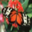
\includegraphics[width=0.64cm,height=0.64cm]{assets/butterfly.png}};
\draw[draw=Flow,line width=0.7pt,line join=round,-{Stealth[length=3.7pt,width=3pt]}] (10.48,6.93) -- (10.780000000000001,6.93);
\draw[fill=SlabTop,draw=SlabEdge,line width=0.25pt,line join=round] (10.9,6.619999999999999) -- (10.975,6.545) -- (11.135,6.545) -- (11.06,6.619999999999999) -- cycle;
\draw[fill=SlabSide,draw=SlabEdge,line width=0.25pt,line join=round] (11.06,6.619999999999999) -- (11.135,6.545) -- (11.135,7.164999999999999) -- (11.06,7.24) -- cycle;
\draw[fill=SlabFace,draw=White,line width=0.52pt] (10.9,6.619999999999999) rectangle (11.06,7.239999999999999);
\draw[fill=SlabTop,draw=SlabEdge,line width=0.25pt,line join=round] (11.16,6.7299999999999995) -- (11.235,6.654999999999999) -- (11.395,6.654999999999999) -- (11.32,6.7299999999999995) -- cycle;
\draw[fill=SlabSide,draw=SlabEdge,line width=0.25pt,line join=round] (11.32,6.7299999999999995) -- (11.395,6.654999999999999) -- (11.395,7.055) -- (11.32,7.13) -- cycle;
\draw[fill=SlabFace,draw=White,line width=0.52pt] (11.16,6.7299999999999995) rectangle (11.32,7.13);
\draw[fill=SlabTop,draw=SlabEdge,line width=0.25pt,line join=round] (11.42,6.619999999999999) -- (11.495000000000001,6.545) -- (11.655000000000001,6.545) -- (11.58,6.619999999999999) -- cycle;
\draw[fill=SlabSide,draw=SlabEdge,line width=0.25pt,line join=round] (11.58,6.619999999999999) -- (11.655000000000001,6.545) -- (11.655000000000001,7.164999999999999) -- (11.58,7.24) -- cycle;
\draw[fill=SlabFace,draw=White,line width=0.52pt] (11.42,6.619999999999999) rectangle (11.58,7.239999999999999);
\draw[draw=Snow,line width=0.7pt,line join=round] (10.995000000000001,6.59) -- (11.145,6.59);
\draw[draw=Snow,line width=0.48pt,line join=round] (11.02125,6.59) -- (11.040341883092037,6.570908116907963);
\draw[draw=Snow,line width=0.48pt,line join=round] (11.02125,6.59) -- (11.040341883092037,6.609091883092036);
\draw[draw=Snow,line width=0.48pt,line join=round] (11.11875,6.59) -- (11.099658116907964,6.609091883092036);
\draw[draw=Snow,line width=0.48pt,line join=round] (11.11875,6.59) -- (11.099658116907964,6.570908116907963);
\draw[draw=Snow,line width=0.7pt,line join=round] (11.0325,6.525048094716166) -- (11.1075,6.654951905283832);
\draw[draw=Snow,line width=0.48pt,line join=round] (11.045625000000001,6.547781261565508) -- (11.071704997309805,6.554769375783277);
\draw[draw=Snow,line width=0.48pt,line join=round] (11.045625000000001,6.547781261565508) -- (11.038636885782232,6.573861258875313);
\draw[draw=Snow,line width=0.48pt,line join=round] (11.094375,6.632218738434491) -- (11.068295002690196,6.625230624216723);
\draw[draw=Snow,line width=0.48pt,line join=round] (11.094375,6.632218738434491) -- (11.101363114217769,6.606138741124687);
\draw[draw=Snow,line width=0.7pt,line join=round] (11.1075,6.525048094716166) -- (11.0325,6.654951905283832);
\draw[draw=Snow,line width=0.48pt,line join=round] (11.094375,6.547781261565508) -- (11.101363114217769,6.573861258875313);
\draw[draw=Snow,line width=0.48pt,line join=round] (11.094375,6.547781261565508) -- (11.068295002690196,6.554769375783277);
\draw[draw=Snow,line width=0.48pt,line join=round] (11.045625000000001,6.632218738434491) -- (11.038636885782232,6.606138741124687);
\draw[draw=Snow,line width=0.48pt,line join=round] (11.045625000000001,6.632218738434491) -- (11.071704997309805,6.625230624216723);
\node[text=Muted,font=\fontsize{8.3}{10.0}\selectfont] (n411) at (11.2775,7.55) {CLIP};
\path let \p1=($(n411.east)-(n411.west)$), \p2=($(n411.north)-(n411.south)$) in \pgfextra{\typeout{SIZE|411|\x1|\y2}};
\draw[draw=Flow,line width=0.7pt,line join=round,-{Stealth[length=3.7pt,width=3pt]}] (11.75,6.93) -- (12.05,6.93);
\node[text=Ink,font=\fontsize{8.3}{10.0}\selectfont] (n413) at (11.97,6.57) {$\Delta A_j$};
\path let \p1=($(n413.east)-(n413.west)$), \p2=($(n413.north)-(n413.south)$) in \pgfextra{\typeout{SIZE|413|\x1|\y2}};
\draw[fill=CyanCell1,draw=White,line width=0.24pt] (12.16,6.82) rectangle (12.36,7.04);
\draw[fill=CyanCell3,draw=White,line width=0.24pt] (12.360000000000001,6.82) rectangle (12.56,7.04);
\draw[fill=CyanCell2,draw=White,line width=0.24pt] (12.56,6.82) rectangle (12.76,7.04);
\draw[fill=CyanCell4,draw=White,line width=0.24pt] (12.760000000000002,6.82) rectangle (12.96,7.04);
\draw[fill=GradCell0,draw=White,line width=0.24pt] (12.16,7.09) rectangle (12.426666666666668,7.1899999999999995);
\draw[fill=GradCell2,draw=White,line width=0.24pt] (12.426666666666668,7.09) rectangle (12.693333333333335,7.1899999999999995);
\draw[fill=GradCell1,draw=White,line width=0.24pt] (12.693333333333333,7.09) rectangle (12.96,7.1899999999999995);
\node[text=Muted,font=\fontsize{8.3}{10.0}\selectfont] (n421) at (10.07,7.55) {Local};
\path let \p1=($(n421.east)-(n421.west)$), \p2=($(n421.north)-(n421.south)$) in \pgfextra{\typeout{SIZE|421|\x1|\y2}};
\node[text=Muted,font=\fontsize{8.3}{10.0}\selectfont] (n422) at (12.56,7.55) {Current\\support};
\path let \p1=($(n422.east)-(n422.west)$), \p2=($(n422.north)-(n422.south)$) in \pgfextra{\typeout{SIZE|422|\x1|\y2}};
\draw[fill=HistorySide,draw=HistorySide,line width=0pt,rounded corners=0.025cm] (13.975000000000001,6.545) rectangle (14.615000000000002,7.225);
\draw[fill=White,draw=HistorySide,line width=0.4pt,rounded corners=0.025cm] (13.940000000000001,6.51) rectangle (14.580000000000002,7.1899999999999995);
\node[text=Ink,font=\fontsize{8.3}{10.0}\selectfont] (n425) at (14.260000000000002,6.7299999999999995) {$s_{t-2}$};
\path let \p1=($(n425.east)-(n425.west)$), \p2=($(n425.north)-(n425.south)$) in \pgfextra{\typeout{SIZE|425|\x1|\y2}};
\draw[fill=IndigoCell1,draw=White,line width=0.24pt] (14.010000000000002,6.99) rectangle (14.176666666666668,7.11);
\draw[fill=IndigoCell2,draw=White,line width=0.24pt] (14.176666666666668,6.99) rectangle (14.343333333333334,7.11);
\draw[fill=IndigoCell3,draw=White,line width=0.24pt] (14.343333333333334,6.99) rectangle (14.51,7.11);
\draw[fill=HistorySide,draw=HistorySide,line width=0pt,rounded corners=0.025cm] (14.975000000000001,6.545) rectangle (15.615000000000002,7.225);
\draw[fill=White,draw=HistorySide,line width=0.4pt,rounded corners=0.025cm] (14.940000000000001,6.51) rectangle (15.580000000000002,7.1899999999999995);
\node[text=Ink,font=\fontsize{8.3}{10.0}\selectfont] (n431) at (15.260000000000002,6.7299999999999995) {$s_{t-1}$};
\path let \p1=($(n431.east)-(n431.west)$), \p2=($(n431.north)-(n431.south)$) in \pgfextra{\typeout{SIZE|431|\x1|\y2}};
\draw[fill=IndigoCell2,draw=White,line width=0.24pt] (15.010000000000002,6.99) rectangle (15.176666666666668,7.11);
\draw[fill=IndigoCell3,draw=White,line width=0.24pt] (15.176666666666668,6.99) rectangle (15.343333333333334,7.11);
\draw[fill=IndigoCell2,draw=White,line width=0.24pt] (15.343333333333334,6.99) rectangle (15.51,7.11);
\draw[draw=Flow,line width=0.6pt,line join=round,-{Stealth[length=3.7pt,width=3pt]}] (14.66,6.93) -- (14.850000000000001,6.93);
\draw[draw=Flow,line width=0.7pt,line join=round,-{Stealth[length=3.7pt,width=3pt]}] (15.68,6.93) -- (16.23,6.93);
\draw[fill=IndigoCell1,draw=White,line width=0.24pt] (16.35,6.82) rectangle (16.55,7.04);
\draw[fill=IndigoCell2,draw=White,line width=0.24pt] (16.55,6.82) rectangle (16.75,7.04);
\draw[fill=IndigoCell2,draw=White,line width=0.24pt] (16.75,6.82) rectangle (16.95,7.04);
\draw[fill=IndigoCell3,draw=White,line width=0.24pt] (16.950000000000003,6.82) rectangle (17.150000000000002,7.04);
\draw[draw=Feedback,line width=0.9pt,line join=round] (16.880000000000003,7.15) -- (16.95,7.22) -- (17.1,7.07);
\node[text=Muted,font=\fontsize{8.3}{10.0}\selectfont] (n442) at (14.780000000000001,7.55) {Across rounds};
\path let \p1=($(n442.east)-(n442.west)$), \p2=($(n442.north)-(n442.south)$) in \pgfextra{\typeout{SIZE|442|\x1|\y2}};
\node[text=Ink,font=\fontsize{9.0}{10.7}\selectfont] (n443) at (16.75,7.55) {$H$};
\path let \p1=($(n443.east)-(n443.west)$), \p2=($(n443.north)-(n443.south)$) in \pgfextra{\typeout{SIZE|443|\x1|\y2}};
\draw[draw=Flow,line width=0.7pt,line join=round,-{Stealth[length=3.7pt,width=3pt]},dash pattern=on 2.5pt off 1.8pt] (11.38,7.98) -- (11.38,8.17) -- (13.11,8.17);
\draw[draw=Flow,line width=0.7pt,line join=round,-{Stealth[length=3.7pt,width=3pt]},dash pattern=on 2.5pt off 1.8pt] (15.57,7.98) -- (15.57,8.17) -- (14.010000000000002,8.17);
\draw[fill=TargetLight,draw=Target,line width=0.55pt] (13.559999999999999,8.17) ellipse (0.36cm and 0.26cm);
\node[text=Muted,font=\fontsize{8.3}{10.0}\selectfont] (n447) at (13.56,8.17) {max};
\path let \p1=($(n447.east)-(n447.west)$), \p2=($(n447.north)-(n447.south)$) in \pgfextra{\typeout{SIZE|447|\x1|\y2}};
\draw[draw=Flow,line width=0.7pt,line join=round,-{Stealth[length=3.7pt,width=3pt]},dash pattern=on 2.5pt off 1.8pt] (13.56,8.469999999999999) -- (13.56,8.559999999999999) -- (12.125,8.559999999999999) -- (12.125,8.809999999999999);
\node[text=Ink,font=\fontsize{8.7}{10.399999999999999}\selectfont] (n449) at (12.84,8.36) {$T$};
\path let \p1=($(n449.east)-(n449.west)$), \p2=($(n449.north)-(n449.south)$) in \pgfextra{\typeout{SIZE|449|\x1|\y2}};
\draw[fill=BlueTop,draw=Blue,line width=0.35pt,line join=round] (9.940000000000001,8.82) -- (10.05,8.71) -- (10.75,8.71) -- (10.64,8.82) -- cycle;
\draw[fill=BlueSide,draw=Blue,line width=0.35pt,line join=round] (10.64,8.82) -- (10.75,8.71) -- (10.75,9.41) -- (10.64,9.52) -- cycle;
\draw[fill=BlueLight,draw=Blue,line width=0.45pt] (9.940000000000001,8.82) rectangle (10.64,9.52);
\node[text=Ink,font=\fontsize{11.0}{12.7}\selectfont] (n453) at (10.290000000000001,9.17) {A};
\path let \p1=($(n453.east)-(n453.west)$), \p2=($(n453.north)-(n453.south)$) in \pgfextra{\typeout{SIZE|453|\x1|\y2}};
\draw[draw=White,line width=0.48pt,line join=round] (9.965,8.844999999999999) -- (10.615,8.844999999999999);
\draw[draw=White,line width=0.48pt,line join=round] (9.965,8.844999999999999) -- (9.965,9.495);
\node[text=Muted,font=\fontsize{8.3}{10.0}\selectfont] (n456) at (10.290000000000001,9.8) {Aggregated};
\path let \p1=($(n456.east)-(n456.west)$), \p2=($(n456.north)-(n456.south)$) in \pgfextra{\typeout{SIZE|456|\x1|\y2}};
\draw[draw=Flow,line width=0.7pt,line join=round,-{Stealth[length=3.7pt,width=3pt]}] (10.850000000000001,9.17) -- (11.280000000000001,9.17);
\draw[fill=White,draw=Target,line width=0.52pt,dash pattern=on 2.4pt off 1.8pt,rounded corners=0.04cm] (11.39,8.879999999999999) rectangle (12.860000000000001,9.249999999999998);
\draw[fill=IndigoCell2,draw=IndigoCell2,line width=0.15pt] (11.450000000000001,8.94) rectangle (11.76875,9.19);
\draw[fill=CyanCell3,draw=CyanCell3,line width=0.15pt] (11.793750000000001,8.94) rectangle (12.1125,9.19);
\draw[fill=IndigoCell3,draw=IndigoCell3,line width=0.15pt] (12.137500000000001,8.94) rectangle (12.45625,9.19);
\draw[fill=CyanCell2,draw=CyanCell2,line width=0.15pt] (12.481250000000001,8.94) rectangle (12.8,9.19);
\node[text=Ink,font=\fontsize{9.7}{11.399999999999999}\selectfont] (n463) at (12.125,9.530000000000001) {$g=\nabla_A\mathcal{L}$};
\path let \p1=($(n463.east)-(n463.west)$), \p2=($(n463.north)-(n463.south)$) in \pgfextra{\typeout{SIZE|463|\x1|\y2}};
\draw[draw=Flow,line width=0.7pt,line join=round,-{Stealth[length=3.7pt,width=3pt]}] (13.02,9.17) -- (13.46,9.17);
\draw[fill=FormulaBg,draw=FormulaBorder,line width=0.52pt,dash pattern=on 2.4pt off 1.8pt,rounded corners=0.12cm] (13.56,8.76) rectangle (16.21,9.58);
\node[text=Ink,font=\fontsize{9.2}{10.899999999999999}\selectfont] (n466) at (14.885000000000002,9.17) {$A^{+}=\Pi(A-\eta g)$};
\path let \p1=($(n466.east)-(n466.west)$), \p2=($(n466.north)-(n466.south)$) in \pgfextra{\typeout{SIZE|466|\x1|\y2}};
\draw[draw=Flow,line width=0.7pt,line join=round,-{Stealth[length=3.7pt,width=3pt]}] (16.29,9.17) -- (16.65,9.17);
\draw[fill=StepTop,draw=Step,line width=0.35pt,line join=round] (16.76,8.82) -- (16.87,8.71) -- (17.57,8.71) -- (17.46,8.82) -- cycle;
\draw[fill=StepSide,draw=Step,line width=0.35pt,line join=round] (17.46,8.82) -- (17.57,8.71) -- (17.57,9.41) -- (17.46,9.52) -- cycle;
\draw[fill=StepLight,draw=Step,line width=0.45pt] (16.76,8.82) rectangle (17.46,9.52);
\node[text=Ink,font=\fontsize{11.0}{12.7}\selectfont] (n471) at (17.11,9.17) {$A^{+}$};
\path let \p1=($(n471.east)-(n471.west)$), \p2=($(n471.north)-(n471.south)$) in \pgfextra{\typeout{SIZE|471|\x1|\y2}};
\draw[draw=White,line width=0.48pt,line join=round] (16.785,8.844999999999999) -- (17.435000000000002,8.844999999999999);
\draw[draw=White,line width=0.48pt,line join=round] (16.785,8.844999999999999) -- (16.785,9.495);
\draw[fill=Orange,draw=Orange,line width=0.3pt,line join=round] (16.880000000000003,8.7) -- (16.91,8.77) -- (16.94,8.735) -- (16.975,8.809999999999999) -- (16.965,8.865) -- (16.925,8.9) -- (16.86,8.9) -- (16.815,8.865) -- (16.810000000000002,8.809999999999999) -- (16.845,8.76) -- (16.85,8.82) -- (16.89,8.77) -- cycle;
\draw[fill=OrangeLight,draw=OrangeLight,line width=0.15pt,line join=round] (16.865000000000002,8.879999999999999) -- (16.915,8.879999999999999) -- (16.906,8.83) -- (16.89,8.844999999999999) -- (16.886000000000003,8.802) -- cycle;
\node[text=Muted,font=\fontsize{8.3}{10.0}\selectfont] (n476) at (17.11,9.8) {Refined};
\path let \p1=($(n476.east)-(n476.west)$), \p2=($(n476.north)-(n476.south)$) in \pgfextra{\typeout{SIZE|476|\x1|\y2}};
\draw[draw=Flow,line width=0.6pt,line join=round,-{Stealth[length=3.7pt,width=3pt]},dash pattern=on 2.5pt off 1.8pt] (17.58,9.17) -- (17.71,9.17) -- (17.71,6.91) -- (17.25,6.91);
\draw[draw=Flow,line width=0.7pt,line join=round,-{Stealth[length=3.7pt,width=3pt]}] (2.2,10.43) -- (2.68,10.43);
\node[text=Muted,font=\fontsize{8.3}{10.0}\selectfont] (n479) at (3.89,10.43) {Model flow};
\path let \p1=($(n479.east)-(n479.west)$), \p2=($(n479.north)-(n479.south)$) in \pgfextra{\typeout{SIZE|479|\x1|\y2}};
\draw[draw=Flow,line width=0.7pt,line join=round,-{Stealth[length=3.7pt,width=3pt]},dash pattern=on 2.5pt off 1.8pt] (5.45,10.43) -- (5.93,10.43);
\node[text=Muted,font=\fontsize{8.3}{10.0}\selectfont] (n481) at (7.14,10.43) {Feedback};
\path let \p1=($(n481.east)-(n481.west)$), \p2=($(n481.north)-(n481.south)$) in \pgfextra{\typeout{SIZE|481|\x1|\y2}};
\draw[draw=Snow,line width=0.7pt,line join=round] (8.96,10.43) -- (9.16,10.43);
\draw[draw=Snow,line width=0.48pt,line join=round] (8.995000000000001,10.43) -- (9.020455844122717,10.404544155877284);
\draw[draw=Snow,line width=0.48pt,line join=round] (8.995000000000001,10.43) -- (9.020455844122717,10.455455844122715);
\draw[draw=Snow,line width=0.48pt,line join=round] (9.125,10.43) -- (9.099544155877284,10.455455844122715);
\draw[draw=Snow,line width=0.48pt,line join=round] (9.125,10.43) -- (9.099544155877284,10.404544155877284);
\draw[draw=Snow,line width=0.7pt,line join=round] (9.01,10.343397459621556) -- (9.110000000000001,10.516602540378443);
\draw[draw=Snow,line width=0.48pt,line join=round] (9.0275,10.373708348754011) -- (9.062273329746406,10.383025834377701);
\draw[draw=Snow,line width=0.48pt,line join=round] (9.0275,10.373708348754011) -- (9.01818251437631,10.408481678500417);
\draw[draw=Snow,line width=0.48pt,line join=round] (9.092500000000001,10.486291651245988) -- (9.057726670253595,10.476974165622298);
\draw[draw=Snow,line width=0.48pt,line join=round] (9.092500000000001,10.486291651245988) -- (9.101817485623691,10.451518321499583);
\draw[draw=Snow,line width=0.7pt,line join=round] (9.110000000000001,10.343397459621556) -- (9.01,10.516602540378443);
\draw[draw=Snow,line width=0.48pt,line join=round] (9.092500000000001,10.373708348754011) -- (9.101817485623691,10.408481678500417);
\draw[draw=Snow,line width=0.48pt,line join=round] (9.092500000000001,10.373708348754011) -- (9.057726670253595,10.383025834377701);
\draw[draw=Snow,line width=0.48pt,line join=round] (9.0275,10.486291651245988) -- (9.01818251437631,10.451518321499583);
\draw[draw=Snow,line width=0.48pt,line join=round] (9.0275,10.486291651245988) -- (9.062273329746406,10.476974165622298);
\node[text=Muted,font=\fontsize{8.3}{10.0}\selectfont] (n497) at (10.15,10.43) {Frozen};
\path let \p1=($(n497.east)-(n497.west)$), \p2=($(n497.north)-(n497.south)$) in \pgfextra{\typeout{SIZE|497|\x1|\y2}};
\draw[fill=Orange,draw=Orange,line width=0.3pt,line join=round] (11.789000000000001,10.32) -- (11.822000000000001,10.397) -- (11.855,10.3585) -- (11.893500000000001,10.440999999999999) -- (11.8825,10.5015) -- (11.838500000000002,10.54) -- (11.767000000000001,10.54) -- (11.717500000000001,10.5015) -- (11.712000000000002,10.440999999999999) -- (11.7505,10.386) -- (11.756,10.452) -- (11.8,10.397) -- cycle;
\draw[fill=OrangeLight,draw=OrangeLight,line width=0.15pt,line join=round] (11.7725,10.517999999999999) -- (11.8275,10.517999999999999) -- (11.8176,10.463) -- (11.8,10.4795) -- (11.7956,10.4322) -- cycle;
\node[text=Muted,font=\fontsize{8.3}{10.0}\selectfont] (n500) at (13.14,10.43) {Trainable};
\path let \p1=($(n500.east)-(n500.west)$), \p2=($(n500.north)-(n500.south)$) in \pgfextra{\typeout{SIZE|500|\x1|\y2}};
\end{tikzpicture}
\end{document}
